\chapter{Claim Clustering}
\label{chap:argclu}

% TODO think about having an example with equivalent claims 
%expressed differently

We will start analyzing discussions by trying to find the discussions' most prominent 
claims.
When discussing a topic, users express claims to back up their opinion. 
Recognizing claims in text is a challenge in online discussions due to 
dealing with noisy, vague, and implicit text. 
Users use claims are to form arguments. 
Arguments can then lead to more complex 
argumentation structures, such as argumentation schemes \citep{walton2008argumentation}. 
But, forming arguments from claims and generally going above the claim level of
argumentation abstraction is beyond the scope of this thesis. 
As a first step of argumentation analysis, we wish to explore how prominent
claims can be detected using standard methods which combine natural language
processing and unstructured machine learning. 

In this chapter, we will first investigate on how to find 
prominent claim candidates from text, considering the variability on how 
claims can be expressed. Second, we investigate the possibility of 
acquiring prominent claims from an online discussion by means of clustering, 
setting a baseline for unsupervised prominent claim identification. 
We will start by introducing the dataset used to study clustering of
user comments to determine prominent claims in section~\ref{sec:argclu_data}.
Next, we will introduce an unsupervised
model for claim clustering in section~\ref{sec:argclu_model}.
The results of the model will be analyzed in section~\ref{sec:argclu_analysis}.
Finally, we will conclude in section~\ref{sec:argclu_conclusion}. 

\section{Data}
\label{sec:argclu_data}

We conduct our study on the dataset of users' posts compiled by \citet{hasan2014you}. 
The dataset is acquired from two-side online debate forums on four topics: 
``Obama'', ``Marijuana'', ``Gay rights'', and ``Abortion''.
Each post is assigned a stance label (\textit{\textcolor{green}{pro}} or 
\textit{\textcolor{red}{con}}), provided
by the author of the post. 
Furthermore, each post is split up into sentences and each sentence is manually labelled
with one prominent claim from a predefined set of prominent claims 
(different for each topic). 
All sentences are argumentative, non-argumentative sentences were removed from the 
dataset (ratio of argumentative sentences topically varies from  20\% to 43.7\%). 
\citet{hasan2014you} report high levels of inter-annotator agreement (between
0.61 and 0.67 $\kappa$). 
Additionally, sentences with rarely occuring prominent claims ($<2\%$) were removed. 
In the end, the dataset contains 3104 sentences (``Abortion'' 814, ``Gay rights'' 824, 
``Marijuana'' 836, and ``Obama'' 630) and 47 different prominent claims
(25 \textit{\textcolor{green}{pro}} and 22 \textit{\textcolor{red}{con}}, an
average of 12 prominent claims per topic).  Majority of sentences (2028
sentences) are labelled with \textit{\textcolor{green}{pro}} prominent claims.
The average sentence length is 14 words. 

\section{Model}
\label{sec:argclu_model}

We use two approaches to measuring similarity of claims. 
%\paragraph{Vector space similarity. } 
We represent sentences as vectors in a semantic space. 
We use two represetations 
\begin{enumerate} 
\item a bag-of-word (BoW) vector, weighted
by inverse sentence frequency and 
\item a distributed representation based on the skip-gram model
	\citep{mikolov2013distributed}. 
\end{enumerate}
These methods of representing sentences are explained in more detail in 
section~\ref{sec:word_representations}. 
We use BoW as it has been shown to be a powerful baseline for semantic similarity 
\citep{ramage2009random}. 
Using weighing by inverse sentence frequency is similar to the motivation 
of inverse-document frequency in tf-idf (described in section~\ref{sec:word_representations} and
equation~\ref{eq:idf}), which is that more frequently used words are less
specific to a prominent claim, thus contributing less to similarity. 
Distributed representations were chosen since they represent individual words 
very well (as shown in \citep{mikolov2013efficient, mikolov2013distributed}).
To build a sentence vector, we simply sum up the distributed vector representations 
of words\footnote{we use pretrained vectors from \url{https://code.google.com/archive/p/word2vec/}}
For both representations, we remove stopwords before building vectors. 
Similarity between sentences is computed as cosine similarity between 
respective sentence vectors. 
As described in section~\ref{sec:sts} we use TakeLab's STS, which we feed our pairs
of claims to acquire a similarity score. 

For clustering we use the hierarchical agglomerative clustering (HAC) algorithm
(described in section~\ref{sec:hierarhical_clustering}). 
There are three main reasons to use HAC: 
\begin{enumerate*}
\item HAC allows us to work directly with similarities
coming from the STS systems, instead of requiring explicit vector-space representations, 
\item HAC produces hierarhical structures, allowing to investigate
granularity of claims, and
\item HAC is a deterministic algorithm, making the results more stable.
\end{enumerate*}
HAC works with a distance matrix computed for all pairs of instances. 
We compute this matrix for all pairs of sentences $s_1$ and $s_2$ and 
compute vector-space similarity with: 
$$
\mathit{vs_{sim}} = 1 - \cos(v_1, v_2)
$$ 
where $v_1$ and $v_1$ are vectors for sentences $s_1$ and $s_2$ respectively.
STS similarity is computed as:
$$
\mathit{sts_{sim}} = \frac{1}{1 + \mathit{sim}(s_1, s_2)}
$$
where $\mathit{sim}(s_1, s_2)$ is a method that returns the STS similarity
between sentences $s_1$ and $s_2$. 
As for linkage, we use complete linkage and Ward's method \citep{ward1963hierarchical}. 
We do not cluster \textit{pro} and \textit{con} sentences separately. 
This allows us to investigate to which extent stance can be captured by 
semantic similarity (and is also more realistic). 

\section{Claim Cluster Analysis}
\label{sec:argclu_analysis}

Using data from online discussions presented in the previous section, 
we wish to cluster posts and analyze the subsequent results. 
We perform two kinds of analysis. First, we analyze different clustering models. 
Second, we analyze clustering quality from one the clustering models chosen. 
To evaluate clustering results, we adopt the external evaluation approach, which compares the 
hypothesized clusters against target clusters. 
We use argument labels from \citet{hasan2014you} as target clusters. 
As a metric of measurement, we use two metrics: 
adjusted rand index (ARI) 
\citep{steinley2004properties}, and V-measure \citep{rosenberg2007v}
(methods described in section~\ref{sec:clus_evaluation}, more specifically by equations
~\ref{eq:adjusted_rand_index} and~\ref{eq:v-measure}). 

\begin{table*}[t]
\begin{center}
{\footnotesize
\setlength{\tabcolsep}{0.5em}
\begin{tabular}{@{}l cccc cccc cccc cccc@{}}
\toprule
& \multicolumn{4}{c}{``Obama''} & \multicolumn{4}{c}{``Marijuana''} &
	\multicolumn{4}{c}{``Gay rights''} & \multicolumn{4}{c}{``Abortion''}
	\\
\cmidrule(lr){2-5}
\cmidrule(lr){6-9}
\cmidrule(lr){10-13}
\cmidrule(lr){14-17}
Model (linkage) &
$h$ & $c$ & $V$ & ARI &
$h$ & $c$ & $V$ & ARI &
$h$ & $c$ & $V$ & ARI &
$h$ & $c$ & $V$ & ARI \\
\midrule
BoW (Complete) &
.15 & .15 & .15 & .03 & 
.04 & .04 & .04 & .00 & 
.04 & .04 & .04 & .01 & 
.05 & .04 & .04 & .01\\
%.153 & .150 & .152 & .025 & 
%.040 & .036 & .038 & .002 & 
%.039 & .036 & .038 & .007 & 
%.045 & .041 & .043 & .005\\
BoW (Ward's) & 
.22 & \textbf{.34} & .27 & .04 & 
.15 & .20 & .17 & .02 & 
.13 & \textbf{.17} & \textbf{.15} & .04 & 
.22 & \textbf{.27} & \textbf{.24} & .07 \\
%.218 & .342 & .266 & .042 & 
%.145 & .197 & .167 & .016 & 
%.127 & .169 & .145 & .038 & 
%.223 & .266 & .243 & .072 \\
Skip-gram (Complete) & 
.18 & .26 & .21 & .04 & 
.09 & .22 & .13 & .02 & 
.09 & .10 & .10 & .04 & 
.17 & .24 & .20 & .03  \\
%.177 & .261 & .211 & .041 & 
%.094 & .216 & .131 & .021 & 
%.089 & .104 & .096 & .043 & 
%.167 & .242 & .198 & .026  \\
Skip-gram (Ward's) & 
\textbf{.30} & .29 & \textbf{.30} & \textbf{.10} & 
\textbf{.25} & \textbf{.24} & \textbf{.25} & \textbf{.19} & 
\textbf{.16} & .15 & \textbf{.15} & \textbf{.07} & 
\textbf{.24} & .22 & .23 & \textbf{.08} \\
%.300 & .294 & .297 & .102 & 
%.250 & .242 & .246 & .186 & 
%.156 & .152 & .154 & .072 & 
%.235 & .217 & .226 & .078 \\
STS (Complete) & .11 & .11 & .11 & .02 & .05 & .05 & .05 & .03	& .05 & .05 & .05 & .01 & .06 & .06 & .06 & .02

 \\
\bottomrule
\end{tabular}}
\caption{External evaluation of clustering models on the four topics using 
	homogeneity ($h$), completeness ($c$), V-measure ($V$), and adjusted
	Rand index (ARI) }
\label{tab:external-eval}
\end{center}
\end{table*}

\paragraph{Analysis \rom{1}} 
For the first analysis, we cluster sentences from four topics separately. 
and use the gold number of clusters for each topic. 
Results are shown in table~\ref{tab:external-eval}. 
Overall, the best model is skip-gram with Ward's linkage 
outperforming in both ARI and V-measure. 
That model also produces best clusters in terms of homogeneity and 
completeness. 
Ward's linkage seems to work better than complete for both BoW and skip-gram models, whereas
the model using STS behaves comparable to baseline results. 
The reason for poor performance of the STS model might lie in the
the fact that STS was trained 
on different domains, and does not model the claim similarity we seek here.  
Furthermore, there is a lot of variance across different topics. 
This is supported by the fact that claims from ``Gay rights'' seem most
difficult to cluster, whereas claims from the 
``Marijuana'' topic seem to be the easiest to cluster with significant ($>50\%$) differences 
In subsequent experiments, we focus on the skip-gram model 
with Ward's linkage and the ``Marijuana'' topic. 

\begin{table*}[ht]
\setlength{\tabcolsep}{0.4em}
{\scriptsize
\begin{center}
\begin{tabular}{lp{3.8em}p{33.0em}|lp{3.8em}p{10em}}
\toprule
\multicolumn{3}{c}{Hypothesized clustering} & \multicolumn{3}{c}{Gold classes}\\
\cmidrule(lr){1-3}\cmidrule(lr){4-6}
Id & Classes & Cluster medoid & Id & Clusters & Gold prominent claim \\
\midrule
1 &  \textbf{10 (54\%)}  \newline  2 (12\%)  \newline  6 (10\%)  &

\str{%
Tobacco and alcohol are both legal and widely used in the US, (...) If the abuse of marijuana is harmful, isn't the abuse of tobacco or alcohol equally life threatening? (...)
} &

1  &  5 (23\%) \newline 9 (19\%) \newline 10 (18\%) 
&
\str{%
%I would argue that marijuana should be illegal as long as all other drugs are illegal, but then again, marijuana has actually treated people with anorexia and helped other people with loss of appetite.
Used as a medicine for its positive effects
}
\\
\midrule
2 & \textbf{4 (92\%) } \newline  9 (8\%) &
\str{%
The biggest effect would be an end to brutal mandatory sentencing of long jail times that has ruined so many young peoples lives.
} 
& 
2  &  1 (33\%) \newline 9 (28\%) \newline 3 (15\%) 
&
\str{%
%(...) I think it ridiculous that people want to legalise something that has four - seven times the amount of tar (the cancer causing agent) in one cone than in one cigarette (...)
Responsible for brain damage
}

\\
\midrule
3 &  \textbf{9 (44\%)}  \newline  4 (25\%)  \newline 7 (8\%) &
\str{%
Legalizing pot alone would not end the war on drugs. It would help (...) my personal opinion would be the only way to completely end the war on drugs would be to legalize everything. 
} 
& 3  &  9 (41\%) \newline 3 (23\%) \newline 10 (23\%) 
&
\str{%
%Worst case scenario, half the population would go out and buy it, get high and wreak havoc on America. Productivity would go down :) and some people would simply do reckless things.
Causes crime
}

\\
\midrule
4 &  \textbf{8 (37\%)}  \newline  1 (22\%)  \newline  10 (17\%)   & 
\str{%
What all these effects have in common is that they result from changes in the brain's control centers (...) So, when marijuana disturbs functions centered in the deep control centers, disorienting changes in the mind occur (...)
} &
4  &  9 (40\%) \newline 3 (26\%) \newline 10 (12\%)  
&
\str{%
%it is not the governments place to control personal aspects of my life that would have no affect on anyone else.
Prohibition violates human rights
}
\\
\midrule
5 &  \textbf{1 (45\%)}  \newline  6 (18\%)  \newline  8 (10\%)  & 
\str{%
People with pre-existing mental disorders also tend to abuse alcohol and tobacco. (...) the link between marijuana use and mental illness may be an instance when correlation does not equal causation. 
} 
&
5  &  6 (25\%) \newline 7 (25\%) \newline 4 (18\%) 
&
\str{%
%you also have to consider that continuous usage of LSD can cause severe mental illnesses in people. There hasn't ever been a case of this happening from using marijuana.
Does not cause any damage to our bodies
}
\\
\midrule
6 &  \textbf{5 (63\%)}  \newline  10 (31\%)  \newline  1 (6\%) & 
\str{%
There are thousands of deaths every year from tobacco and alcohol, yet there has never been a recorded death due to marijuana.
} &
6  &  9 (29\%) \newline 1 (19\%) \newline 7 (16\%) 
&
\str{%
%There have been many deaths directly linked to marijuana use. Car crashes are a common way in which people under the influence of marijuana harm themselves, and others.
Damages our bodies
}
\\
\midrule
7 &  \textbf{10 (48\%)}  \newline  5 (13\%)  \newline  6 (12\%)    &
\str{%
as far as it goes for medicinal purposes, marijuana does not cure anything (...) It is for the sole purpose of numbing the pain in cancer patients (...) and also making patients hungry so they eat more and gain weight on their sick bodies 
} &
7  &  9 (39\%) \newline 3 (30\%) \newline 1 (9\%) 
&
\str{%
%The last thing we need is more people doing it. More people making it a problem for themselves, more people ending up in rehab at the governments expense.
Highly addictive
}
\\
\midrule
8 &  \textbf{9 (92\%)} &
\str{%
the economy would get billions of dollars in a new industry if it were legalized (...) no longer would this revenue go directly into the black market.
} 
&
8  &  4 (44\%) \newline 7 (16\%) \newline 9 (16\%) 
&
\str{%
%If we legalize something that makes people stop caring about their lives and only want to get "high" then we are pretty much setting a course for our downfall as a civilization.
If legalized, people will use marijuana and other drugs more
}
\\
\midrule
9 &  \textbf{4 (30\%)}  \newline  9 (13\%)  \newline  10 (11\%)   &
\str{%
(...) I think it ridiculous that people want to legalise something that has four - seven times the amount of tar (the cancer causing agent) in one cone than in one cigarette (...)
} &
9  &  8 (53\%) \newline 3 (25\%) \newline 9 (10\%) 
&
\str{%
%Not only would it be better for the economy, but look at Amsterdam - weed is legal over there and you never hear anything out of them. They've been onto something for a long time now.
Legalized marijuana can be controlled and regulated by the government
}
\\
\midrule
10 &  \textbf{10 (30\%)}  \newline  9 (19\%)  \newline  4 (15\%)   &
\str{%
But I'm not gonna tell anyone they can't smoke pot or do meth because I don't like it.
} &
10  &  1 (36\%) \newline 7 (21\%) \newline 10 (18\%) 
& 
\str{%
%I don't personally use it, or have any real want to, but I don't think it's any worse than alcohol or cigarettes.
Not addictive
}
 \\
\bottomrule
\end{tabular}
\caption{Manual cluster-class matching for the ``Marijuana'' topic and the gold
number of clusters}
\label{tab:cluster-class}
\end{center}}
\end{table*}

\begin{table*}
\setlength{\tabcolsep}{0.4em}
{\scriptsize
\begin{center}
\begin{tabular}{@{}lp{19em} p{16em} p{16em}@{}}
\toprule
Id & Statement & Hypothesized clustering argument & Gold argument \\
\midrule
\#knowledge  & 
\str{%
Pot is also one of the most high priced exports of Central American Countries and the Carribean}
& 
\str{%
Not addictive
}
& 
\str{%
Legalized marijuana can be controlled and regulated by the government} 
\\
\midrule
\#colloquial & 
\str{%
If I want to use pot, that is my business!}
& 
\str{%
Legalized marijuana can be controlled and regulated by the government} &
\str{%
Prohibition violates human rights}
\\
\midrule
\#opposing & 
\str{%
(...) immediately following the legalization of the drug would cause widespread pandemonium. (...)
} 
& 
\str{%
Legalized marijuana can be controlled and regulated by the government
} & 
\str{%
If legalized, people will use marijuana and other drugs more }
\\
\midrule
\#general & 
\str{%
The user's psychomotor coordination becomes impaired (...), narrow attention span, "depersonalization, euphoria or depression (...)
}
& 
\str{%
Damages our bodies
}
& 
\str{%
Responsible for brain damage
} 
\\
%3 & 
%\str{%
%You're right that not many people ask where their stuff is from but even the dealer has a duty to the buyer to expose a heavy additive
%}
% & 
%\str{%
%Prohibition violates human rights
%} &
%\str{%
% Highly addictive} 
%  \\
%\#specific & 
%\str{%
%People who are already obese would get the munchies and that would make matters worse.
%} &
%\str{%
%If legalized, people will use marijuana and other drugs more.
%} &
%\str{%
%Highly addictive
%}
%\\
%10  & 
%\str{%
%Sure it makes you sleepy and hungry but it also makes you happy!} & 
%\str{%
%Used as a medicine for its positive effects}
%& \str{%
%Does not cause any damage to our bodies}
%\\
%\#rhetorical & 
%\str{%
%Who are you to tell me what I ingest?   If I want to snort cocaine, why can't I?} &
%\str{%
%Legalized marijuana can be controlled and regulated by the government
% }
% & 
% \str{%
% Prohibition violates human rights
% }
% \\
\bottomrule
\end{tabular}
\caption{Error analysis examples for the ``Marijuana'' topic}
\label{tab:err-analysis}
\end{center}}
\end{table*}

\paragraph{Analysis \rom{2}.} 
Now, we focus on analyzing how well the clusters match to gold 
prominent claims. 
We manually attempt to match resulting clusters from 
the skip-gram model with Ward's linkage for the ``Marijuana'' topic configured
to produce 10 clusters (which is the number of gold prominent claims). 
We do matching on the majority basis, which matches 6 gold classes. 
Results are shown in table~\ref{tab:cluster-class}. 
We list top three gold classes (and the percentage of sentences in the dataset) 
in each predicted cluster and top three
(and the percentage of sentences) in each of the gold classes. 
Two gold classes  ($\#4$ and $\#9$) frequently co-occur, indicating 
that they are similar. 
We characterize each cluster by its medoid (the sentence closest to cluster centroid)

\paragraph{Error analysis.}
Grouping statements into coherent clusters is challenging. 
While analyzing the errors, We notice that the main problems are related to \begin{enumerate*}
\item the need for background knowledge, 
\item use of idiomatic language, 
\item grammatical errors, 
\item opposing claims, and 
\item too fine/coarse gold claims.
\end{enumerate*}
Table~\ref{tab:err-analysis} shows a sample of errors. 
Example \#knowledge demonstrates the need for background knowledge 
(exports are government regulated). 
A colloquial expression (\emph{pot}) is used in example \#colloquial. 
In example \#oppose, the statement is assigned to cluster of the opposite-stance
claim. 
And finally, in example \#general our model predicts are a more coarse claim. 

\begin{figure}[h]
\begin{center}
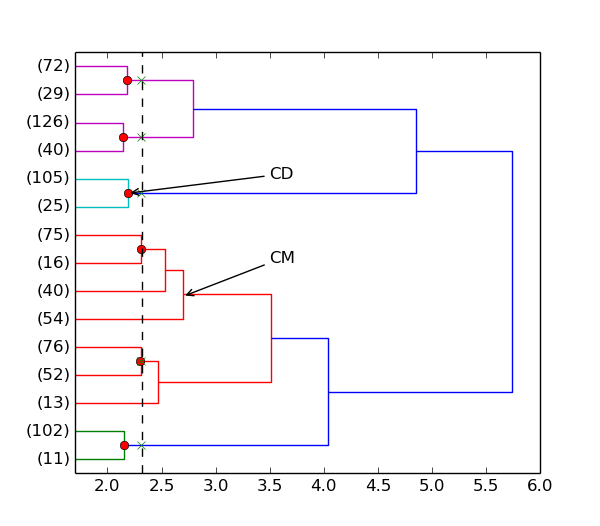
\includegraphics{dendrogram.png}
\end{center}
\caption{Dendrogram for applying HAC (last 15 steps) on the ``Marijuana'' topic.
The dashed line shows the 10-clusters cut, which is number of gold prominent
claims.
CM denotes a merger of clusters that consist mostly of two prominent claims: 
\textit{Damages our bodies} and \textit{Responsible for brain damage}.  \\
In CD there is a split between clusters represented by medoids with: 
item \textit{the economy would get billions of dollars (...) no longerwould this revenue
go directly into the black market} and 
\textit{If the tax on cigarettes can
be \$5.00/pack imagine what we could tax pot for!}
}
\label{fig:dendrogram}
\end{figure}

In the previous analysis we used the gold number of prominent claims to compare
against. However, we note that claim granularity is something arbitrary. 
We exemplify this with example~\ref{fig:dendrogram} where the last 15 steps of
hierarchical agglomerative clustering. 
Looking at the dendrogram point CD there is a split between clusters represented by medoids with: 
\begin{enumerate*}[label=\arabic*)]
\item \textit{the economy would get billions of dollars (...) no longerwould this revenue
go directly into the black market} and 
\item \textit{If the tax on cigarettes can
be \$5.00/pack imagine what we could tax pot for!}
\end{enumerate*}
These clusters could have been treated as separate prominent claims about
economy and tax. 
On the other hand, dendrogram point CM denotes a merger of clusters that
consist mostly of two prominent claims: 
\begin{enumerate*}[label=\arabic*)]
\item \textit{Damages our bodies} and 
\item \textit{Responsible for brain damage}.
\end{enumerate*}
These could have been represented as a single prominent claim which would state: 
\textit{Damaging our entire bodies}. 
The dendrogram also suggests that having 10 prominent claims might not be optimal 
for the ``Marijuana'' topic and the similarity measure. 

\section{Conclusion}
\label{sec:argclu_conclusion}

In this chapter, we explored one of the first steps to performing argumentation
mining of claims: clustering claims to determine prominent claim candidates.
More specifically, we used hierarchical agglomerative clustering (HAC) to
claims in online discussions by clustering semantically similar sentences.  The
best performing clustering models achieved 0.15 to 0.30 V-measure. 
We noticed that  there seem to be differences that basic textual similarity
can't measure, as textual similarity might be too much on the surface level. 

Claim clustering is one possible, unstructured, approach to 
detect prominent claims from text  
It is unstructured, as we do not know anything, but the final result of
prominent claims. In part~\ref{part:struc} of the thesis, we will provide an
alternative perspective on clustering claims to derive prominent claims: a
structured approach involving formalizations and reasoning. This unstructured
approach does not allow for describing relationships between resulting
prominent claims. Thus, we move on the next chapter, where we will 
explore determining the relationships between claims through the 
prominent claim identification task. 

